\documentclass{tufte-handout}

%\geometry{showframe}% for debugging purposes -- displays the margins

\usepackage{amsmath,amsthm,amssymb}
\theoremstyle{definition}
\newtheorem{theorem}{Theorem}[section]
\newtheorem*{theorem*}{Theorem}
\newtheorem{corollary}[theorem]{Corollary}
\newtheorem{lemma}[theorem]{Lemma} 
\newtheorem{proposition}[theorem]{Proposition}
\newtheorem{conj}[theorem]{Conjecture}
\newtheorem{defn}[theorem]{Definition}
\newtheorem{fact}[theorem]{Fact} 
\newtheorem{example}[theorem]{Example} 
\newtheorem{examples}[theorem]{Examples}
\newtheorem{example*}[theorem]{Example*}
\newtheorem{examples*}[theorem]{Examples*}
\newtheorem{remark}[theorem]{Remark}
\newtheorem{remark*}[theorem]{Remark*}
\newtheorem{question}[theorem]{Question}
\newtheorem{assumption}[theorem]{Assumption}
\newtheorem{conjecture}[theorem]{Conjecture}
\newtheorem{convention}[theorem]{Convention}
\newtheorem{justification}[theorem]{Justification} 
\newtheorem{construction}[theorem]{Construction}
\newtheorem{rem}[theorem]{Reminder}
\newtheorem{intuition}[theorem]{Intuition}
\newtheorem{term}[theorem]{Terminology}

\usepackage{tikz-cd}
\usepackage{macros/tikzfig}
\usepackage{macros/quiver}
\input{macros/toprel.tikzstyles}

% Set up the images/graphics package
\usepackage{graphicx}
\setkeys{Gin}{width=\linewidth,totalheight=\textheight,keepaspectratio}
\graphicspath{{graphics/}}

\title{The Category of Topological Relations}
\author[me]{Vincent Wang-Ma\'{s}cianica}
\date{\today}

% The following package makes prettier tables.  We're all about the bling!
\usepackage{booktabs}

% The units package provides nice, non-stacked fractions and better spacing
% for units.
\usepackage{units}

% The fancyvrb package lets us customize the formatting of verbatim
% environments.  We use a slightly smaller font.
\usepackage{fancyvrb}
\fvset{fontsize=\normalsize}

% Small sections of multiple columns
\usepackage{multicol}

% Provides paragraphs of dummy text
\usepackage{lipsum}

% These commands are used to pretty-print LaTeX commands
\newcommand{\doccmd}[1]{\texttt{\textbackslash#1}}% command name -- adds backslash automatically
\newcommand{\docopt}[1]{\ensuremath{\langle}\textrm{\textit{#1}}\ensuremath{\rangle}}% optional command argument
\newcommand{\docarg}[1]{\textrm{\textit{#1}}}% (required) command argument
\newenvironment{docspec}{\begin{quote}\noindent}{\end{quote}}% command specification environment
\newcommand{\docenv}[1]{\textsf{#1}}% environment name
\newcommand{\docpkg}[1]{\texttt{#1}}% package name
\newcommand{\doccls}[1]{\texttt{#1}}% document class name
\newcommand{\docclsopt}[1]{\texttt{#1}}% document class option name

\begin{document}

\maketitle% this prints the handout title, author, and date

\begin{abstract}
Abstract here.
\end{abstract}

\begin{fullwidth}
\section{Introduction}

Primarily, I wanted to see what would happen if we replaced continuous functions between topological spaces with continuous relations. The preimage of a function used in the definition of continuity is a relation, so from a na\"{i}ve perspective this is a generalisation that might simplify. An ulterior motive is to construct a category where I can interpret string diagrams for modal first order logic. For first order logic, normal relations (viewed as a bicategory of relations) suffice, where the regular fragment is chiefly handled by the copy-compare spiders, and negation is interpreted as set complementation. The further addition of topological structure would permit the interpretation of the $\diamond$ modality as a closure operator.

\newthought{Findings:} \textbf{TopRel} is a symmetric monoidal closed category with biproducts. It does not inherit a dagger from \textbf{Rel}. States are arbitrary subsets, and effects are open sets.

\end{fullwidth}

\section{Topological Relations}

\marginnote{
\begin{rem}[Topological Space]
A \emph{topological space} is a pair $(X,\tau)$, where $X$ is a set, and $\tau \subset \mathcal{P}(X)$ are the \emph{open sets} of $X$, such that:
\begin{description}
    \item["nothing" and "everything" are open]  \[\varnothing,X \in \tau\]
    \item[Arbitrary unions of opens are open] \[\{ U_i : i \in I \} \subseteq \tau \Rightarrow \bigcup\limits_{i \in I} U_i \in \tau \]
    \item[Finite intersections of opens are open] $n \in \mathbb{N}$: \[U_1,\cdots, U_n \in \tau \Rightarrow \bigcap\limits_{1\cdots, i , \cdots n} U_i \in \tau\]
\end{description}
\end{rem}
}

\marginnote{
\begin{rem}[Relational Converse]
Recall that a relation $R: S \rightarrow T$ is a subset $R \subseteq S \times T$. \[R^\dag : T \rightarrow S := \{ (t,s) : (s,t) \in R \}\]
\end{rem}
}
\begin{defn}[Topological Relation]\label{defn:toprelation}
A topological relation $R: (X,\tau) \rightarrow (Y,\sigma)$ is a relation $R: X \rightarrow Y$ such that \[U \in \sigma \Rightarrow R^{\dag}(U) \in \tau\] where $\dag$ denotes the relational converse.
\end{defn}

For shorthand, we denote the topology $(X,\tau)$ as $X^{\tau}$. As special cases, we denote the discrete topology on $X$ as $X^{\bullet}$, and the indiscrete topology $X^{\circ}$.

\newpage

\begin{fullwidth}

\section{Topological Relations by examples}

Let's consider three topological spaces and examine the topological relations between them. This way we can build up intuitions, and prove some tool results in the process.

The \textbf{singleton space} consists of a single point which is both open and closed. We denote this space $\bullet$. Concretely, the underlying set and topology is
\[(\{\star\} \ , \ \{\{\star\},\varnothing\})\] 
\ctikzfig{testspaces/singleton}

The \textbf{Sierpi\'{n}ski space} consists of two points, one of which (in yellow) is open, and the other (in cyan) is closed. We denote this space $\mathcal{S}$. Concretely, the underlying set and topology is:
\[\big( \{0,1\} \ , \ \{ \varnothing, \{ 1 \} , \{ 0,1\} \} \big)\]
\ctikzfig{testspaces/sierpinski}

The \textbf{unit square} has $[0,1] \times [0,1]$ as its underlying set.  Open sets are "blobs" painted with open balls. Points, lines, and bounded shapes are closed. We denote this space $\blacksquare$.
\ctikzfig{testspaces/unitsquare}
\end{fullwidth}

\newthought{$\bullet \rightarrow \bullet$:} There are two relations from the singleton to the singleton; the identity relation $\{ (\bullet,\bullet) \}$, and the empty relation $\varnothing$. Both are topological.

\newthought{$\bullet \rightarrow \mathcal{S}$:} There are four relations from the singleton to the Sierpi\'{n}ski space, corresponding to the subsets of $\mathcal{S}$. All of them are topological.


\newthought{$\mathcal{S} \rightarrow \bullet$:}
\marginnote{
\begin{example}[A nontopological relation]\label{ex:nontop}
The relation $\{(0,\bullet)\} \subset \mathcal{S} \times \bullet$ is not a topological relation: the preimage of the open set $\{\bullet\}$ under this relation is the non-open set $\{0\}$.
\end{example}
}
There four candidate relations from the Sierpi\'{n}ski space to the singleton, but as we see in Example \ref{ex:nontop}, not all of them are topological.

\newthought{Now we need some abstraction.} We cannote study the topological relations between the singleton and the unit square case by case. We discover that topological relations out of the singleton indicate arbitrary subsets, and that topological relations into the singleton indicate arbitrary opens.
\marginnote{
\begin{term}
Call a topological relation $\bullet \rightarrow X^\tau$ a \textbf{state} of $X^\tau$, and a topological relation $X^\tau \rightarrow \bullet$ a \textbf{test} of $X^\tau$.
\end{term}

\begin{proposition}\label{prop:states}
States $R: \bullet \rightarrow X^{\tau}$ correspond with subsets of $X$.
\begin{proof}
The preimage $R^\dag(U)$ of a (non-$\varnothing$) open $U \in \tau$ is $\star$ if $R(\star) \cap U$ is nonempty, and $\varnothing$ otherwise. Both $\star$ and $\varnothing$ are open in $\{\star\}^{\bullet}$. $R(\star)$ is free to specify any non-$\varnothing$ subset of $X$. The empty relation handles $\varnothing$ as an open of $X^{\tau}$.
\end{proof}
\end{proposition}

\begin{proposition}\label{prop:tests}
Tests $R: X^\tau \rightarrow \bullet$ correspond with open sets $U \in \tau$.
\begin{proof}
The preimage $R^\dag(\star)$ of $\star$ must be an open set of $X^\tau$ by definition \ref{defn:toprelation}. $R^\dag(\star)$ is free to specify any open set of $X^{\tau}$.
\end{proof}
\end{proposition}
}

\newthought{$\bullet \rightarrow \blacksquare$:} Proposition \ref{prop:states} tells us that there are as many topological relations from the singleton to the unit square as there are subsets of the unit square.

\newthought{$\blacksquare \rightarrow \bullet$:} Proposition \ref{prop:tests} tells us that there are as many topological relations from the unit square to the singleton as there are open sets of the unit square.

\newthought{There are 16 candidate relations $\mathcal{S} \rightarrow \mathcal{S}$ to check.} A case-by-case approach won't scale, so we could instead identify the building blocks of topological relations with the same source and target space.

\newthought{Which relations $X^\tau \rightarrow Y^\sigma$ are always continuous?}

\newthought{The empty relation is always continuous.}
\marginnote{
    \begin{rem}[Empty relation]
    The \textbf{empty relation} $X \rightarrow Y$ relates nothing. It is defined:
    \[ \varnothing \subset X \times Y\]
    \end{rem}
}
\begin{proposition}
\label{prop:emptyrel}
\begin{proof}
The preimage of the empty relation is always $\varnothing$, which is open by definition.
\end{proof}
\end{proposition}

\newthought{Full relations are always continuous}
\marginnote{
    \begin{rem}[Full relation]
    The \textbf{full relation} $X \rightarrow Y$ relates everything to everything. It is all of $X \times Y$.
    \end{rem}
}
\begin{proposition}
\label{prop:fullrel}
\begin{proof}
The preimage of any subset of $Y$ -- open or not -- under the full relation is the whole of $X$, which is open by definition.
\end{proof}
\end{proposition}

\newthought{Full relations restricted to open sets in the source are continuous.}
\begin{proposition}\label{prop:bowtie}
Given an open $U \subseteq X^\tau$, and an arbitrary subset $K \subset Y^\sigma$, the relation $U \times K \subseteq X \times Y$ is open. We call such relations \textbf{bowties}, and we denote such a relation $[U\bowtie K]$, read "$U$ bowtie $K$".
\begin{proof}
Consider an arbitrary open set $V \in \sigma$. Either $V$ and $K$ are disjoint, or they overlap. If they are disjoint, the preimage of $V$ is $\varnothing$, which is open. If they overlap, the preimage of $V$ is $U$, which is open.
\end{proof}
\end{proposition}

\newthought{Continuous functions are always continuous.}
\begin{proposition}\label{prop:func}
If $f: X^\tau \rightarrow Y^\sigma$ is a continuous function, then it is also a continuous relation.
\begin{proof}
Functions are special cases of relations. The relational converse of a function viewed in this way is the same thing as the preimage.
\end{proof}
\end{proposition}

\newthought{The identity relation is always continuous.}
\marginnote{
    \begin{rem}[Identity relation]
    The \textbf{identity relation} $X \rightarrow X$ relates anything to itself. It is defined:
    \[ \{(x,x) : x \in X\} \subseteq X \times X\]
    \end{rem}
}
The identity relation is also the "trivial" continuous map from a space to itself, so this also follows from Proposition \ref{prop:func}.
\begin{proposition}\label{prop:idrel}
\begin{proof}
The preimage of any open set under the identity relation is itself, which is open by assumption.
\end{proof}
\end{proposition}

\newthought{Given two continuous relations $R,S : X^\tau \rightarrow Y^\sigma$, how can we combine them?}\marginnote{
\begin{rem}[Union, intersection, and ordering of relations]
Recall that relations $X \rightarrow Y$ can be viewed as subsets of $X \times Y$. So it makes sense to speak of the union and intersection of relations, and of partially ordering them by inclusion.
\end{rem}
}

\begin{proposition}
If $R,S: X^\tau \rightarrow Y^\sigma$ are continuous relations, so are $R \cap S$ and $R \cup S$.
\begin{proof}
Replace $\square$ with either $\cup$ or $\cap$. For any non-$\varnothing$ open $U \in \sigma$: \[(R \square S)^\dag (U) = R^\dag(U) \square S^\dag(U)\] As $R,S$ are continuous relations, $R^\dag(U),S^\dag(U) \in \tau$, so $R^\dag(U) \square S^\dag(U) = (R \square S)^\dag (U) \in \tau$. Thus $R\square S$ is also a continuous relation.
\end{proof}
\end{proposition}

\begin{corollary}\label{cor:homspace}
Continuous relations $X^\tau \rightarrow Y^\sigma$ are closed under arbitrary union and finite intersection. Hence, continuous relations $X^\tau \rightarrow Y^\sigma$ form a topological space where each relation is an open set on the base space $X \times Y$, where the full relation $X \rightarrow Y$ is "everything", and the empty relation is "nothing".
\end{corollary}

\newthought{A topological basis for spaces of continuous relations}
\marginnote{
\begin{rem}[Topological Basis]
$\mathfrak{b} \subseteq \tau$ is a basis of the topology $\tau$ if every $U \in \tau$ is expressible as a union of elements of $\mathfrak{b}$. Every topology has a basis (itself). Minimal bases are not necessarily unique.
\end{rem}
}

\begin{defn}[Partial Functions]
A \textbf{partial function} $X \rightarrow Y$ is a relation for which each $x \in X$ has at most a single element in its image. In particular, all functions are special cases of partial functions, as is the empty relation.
\end{defn}

\begin{lemma}[Partial functions are a $\cap$-ideal]\label{lem:capideal}
The intersection $f \cap R$ of a partial function $f: X \rightarrow Y$ with any other relation $R: X \rightarrow Y$ is again a partial function.
\begin{proof}
Consider an arbitrary $x \in X$. $R(x) \cap f(x) \subseteq f(x)$, so the image of $x$ under $f \cap R$ contains at most one element, since $f(x)$ contains at most one element.
\end{proof}
\end{lemma}

\begin{lemma}[Any single edge can be extended to a continuous partial function]\label{lem:edgecomplete}
Given any $(x,y) \in X \times Y$, there exists a continuous partial function $X^\tau \rightarrow Y^\tau$ that contains $(x,y)$.
\begin{proof}
Let $\mathcal{N}(x)$ denote some open neighbourhood of $x$ with respect to the topology $\tau$. Then $\{ (z,y) : z \in \mathcal{N}(x) \}$ is a continuous partial function that contains $(x,y)$.
\end{proof}
\end{lemma}

\begin{marginfigure}
\centering
\scalebox{0.5}{\tikzfig{paintingexamples/sierandcanvas2_2}}
\caption{Regions of $\blacksquare$ in the image of the yellow point alone will be coloured yellow, and regions in the image of both yellow and cyan will be coloured green:}
\label{fig:yellowgreen}
\end{marginfigure}

\begin{marginfigure}
\centering
\scalebox{0.5}{\tikzfig{paintingexamples/s2sqzoom}}
\caption{Regions in the image of the cyan point alone cannot be open sets by continuity, so they are either points or lines. Points and lines in cyan must be surrounded by an open region in either yellow or green, or else we violate continuity (open sets in red).}
\label{fig:cyan}
\end{marginfigure}

\begin{proposition}\label{prop:hombasis}
Continuous partial functions form a topological basis for the space $(X \times Y)^{(\tau \multimap \sigma)}$ of continuous relations $X^\tau \rightarrow Y^\sigma$.
\begin{proof}
We will show that every continuous relation $R: X^\tau \rightarrow Y^\sigma$ arises as a union of partial functions. Denote the set of continuous partial functions $\mathfrak{f}$. We claim that:
\[ R = \bigcup\limits_{F \in \mathfrak{f}} (R \cap F) \]
The $\supseteq$ direction is evident, while the $\subseteq$ direction follows from Lemma \ref{lem:edgecomplete}.
By Lemma \ref{lem:capideal}, every $R \cap F$ term is a partial function, and by Corollary \ref{cor:homspace}, continuous.
\end{proof}
\end{proposition}

\newthought{$\mathcal{S} \rightarrow \mathcal{S}$:} We can use Proposition \ref{prop:hombasis} to write out the topological basis of continuous partial functions, from which we can take unions to find all the continuous relations, which we depict in Figure \ref{fig:hassesierpinski}.

\newthought{$\mathcal{S} \rightarrow \blacksquare$:}
Now we use the colour convention of the points in $\mathcal{S}$ to "paint" continuous relations on the unit square "canvas", as in Figures \ref{fig:yellowgreen} and \ref{fig:cyan}. So each continuous relation is a painting, and we can characterise the paintings that correspond to continuous relations $\mathcal{S} \rightarrow \blacksquare$ in words as follows: \texttt{Cyan only in points and lines, and either contained in or at the boundary of yellow or green. Have as much yellow and green as you like.}

\begin{marginfigure}
\centering
\scalebox{0.75}{\tikzfig{paintingexamples/s2sqpainting}}
\caption{A topological relation $\mathcal{S} \rightarrow \blacksquare$: "Flower and critter in a sunny field".}
\label{fig:flower}
\end{marginfigure}

\begin{marginfigure}
\centering
\scalebox{0.75}{\tikzfig{paintingexamples/sq2spainting}}
\caption{A topological relation $\blacksquare \rightarrow \mathcal{S}$: "lmao still math". Black lines and dots indicate gaps.}
\label{fig:shitpost}
\end{marginfigure}

\newthought{$\blacksquare \rightarrow \mathcal{S}$:} The preimage of all of $\mathcal{S}$ must be an open set. So the painting cannot have stray lines or points outside of blobs. The preimage of yellow must be open, so the union of yellow and green in the painting cannot have stray lines or points outside of blobs. Point or line gaps within blobs are ok. Each connected blob can contain any colours in any shapes, subject to the constraint that if cyan appears anywhere, then either yellow or green must occur somewhere. \texttt{Open blobs with no lines or points outside. Yellow and green considered alone is a painting made of blobs with no stray lines or points. If cyan appears anywhere, then either yellow or green have to appear somewhere.}


\begin{figure}\label{fig:hassesierpinski}
\scalebox{0.7}{\tikzfig{testspaces/sierpinskienum}}
\caption{Hasse diagram of all continuous relations from the Sierpi\'{n}ski space to itself. Each relation is depicted left to right, and inclusion order is bottom-to-top. Relations that form the topological basis are boxed.}
\end{figure}

\clearpage

\newthought{One more example for fun: $[0,1] \rightarrow \blacksquare$:} We know how continuous functions from the unit line into the unit square look.
\begin{marginfigure}
\centering
\scalebox{0.5}{\tikzfig{paintingexamples/contline}}
\caption{
continuous functions $[0,1] \rightarrow \blacksquare$ follow the na\"{i}ve notion of continuity: \texttt{"a line one can draw on paper without lifting the pen off the page".}
}
\label{fig:contline}
\end{marginfigure}
\newthought{Then what are the partial continuous functions?} If we understand these, we can obtain all continuous relations by arbitrary unions of the basis. Observe that the restriction of any continuous function to an open set in the source is a continuous partial function. The open sets of $[0,1]$ are collections of open intervals, each of which is homeomorphic to $(0,1)$, which is close enough to $[0,1]$.
%
\begin{marginfigure}
\centering
\scalebox{0.5}{\tikzfig{paintingexamples/contlines}}
\caption{
So a continuous partial function is \texttt{"(countably) many (open-ended) lines, each of which one can draw on paper without lifting the pen off the page."}
}
\label{fig:contline}
\end{marginfigure}
%
\begin{marginfigure}
\centering
\scalebox{0.5}{\tikzfig{paintingexamples/thickbrush}}
\caption{We can control the thickness of the brushstroke, by taking the union of (uncountably) many lines.}
\label{fig:thickbrush}
\end{marginfigure}

\newthought{Any painting is a continuous relation $[0,1] \rightarrow \blacksquare$.} By colour-coding $[0,1]$ and controlling brushstrokes, we can do quite a lot. Now we would like to develop the abstract machinery required to \emph{formally} paint pictures with words.

\begin{marginfigure}
\centering
\scalebox{0.8}{
\includegraphics{figures/paintingexamples/spectrum.png}}
\caption{Assign the visible spectrum of light to $[0,1]$. Colour open sets according to perceptual addition of light, computing brightness by normalising the measure of the open set.}
\end{marginfigure}

\begin{marginfigure}
\centering
\scalebox{0.8}{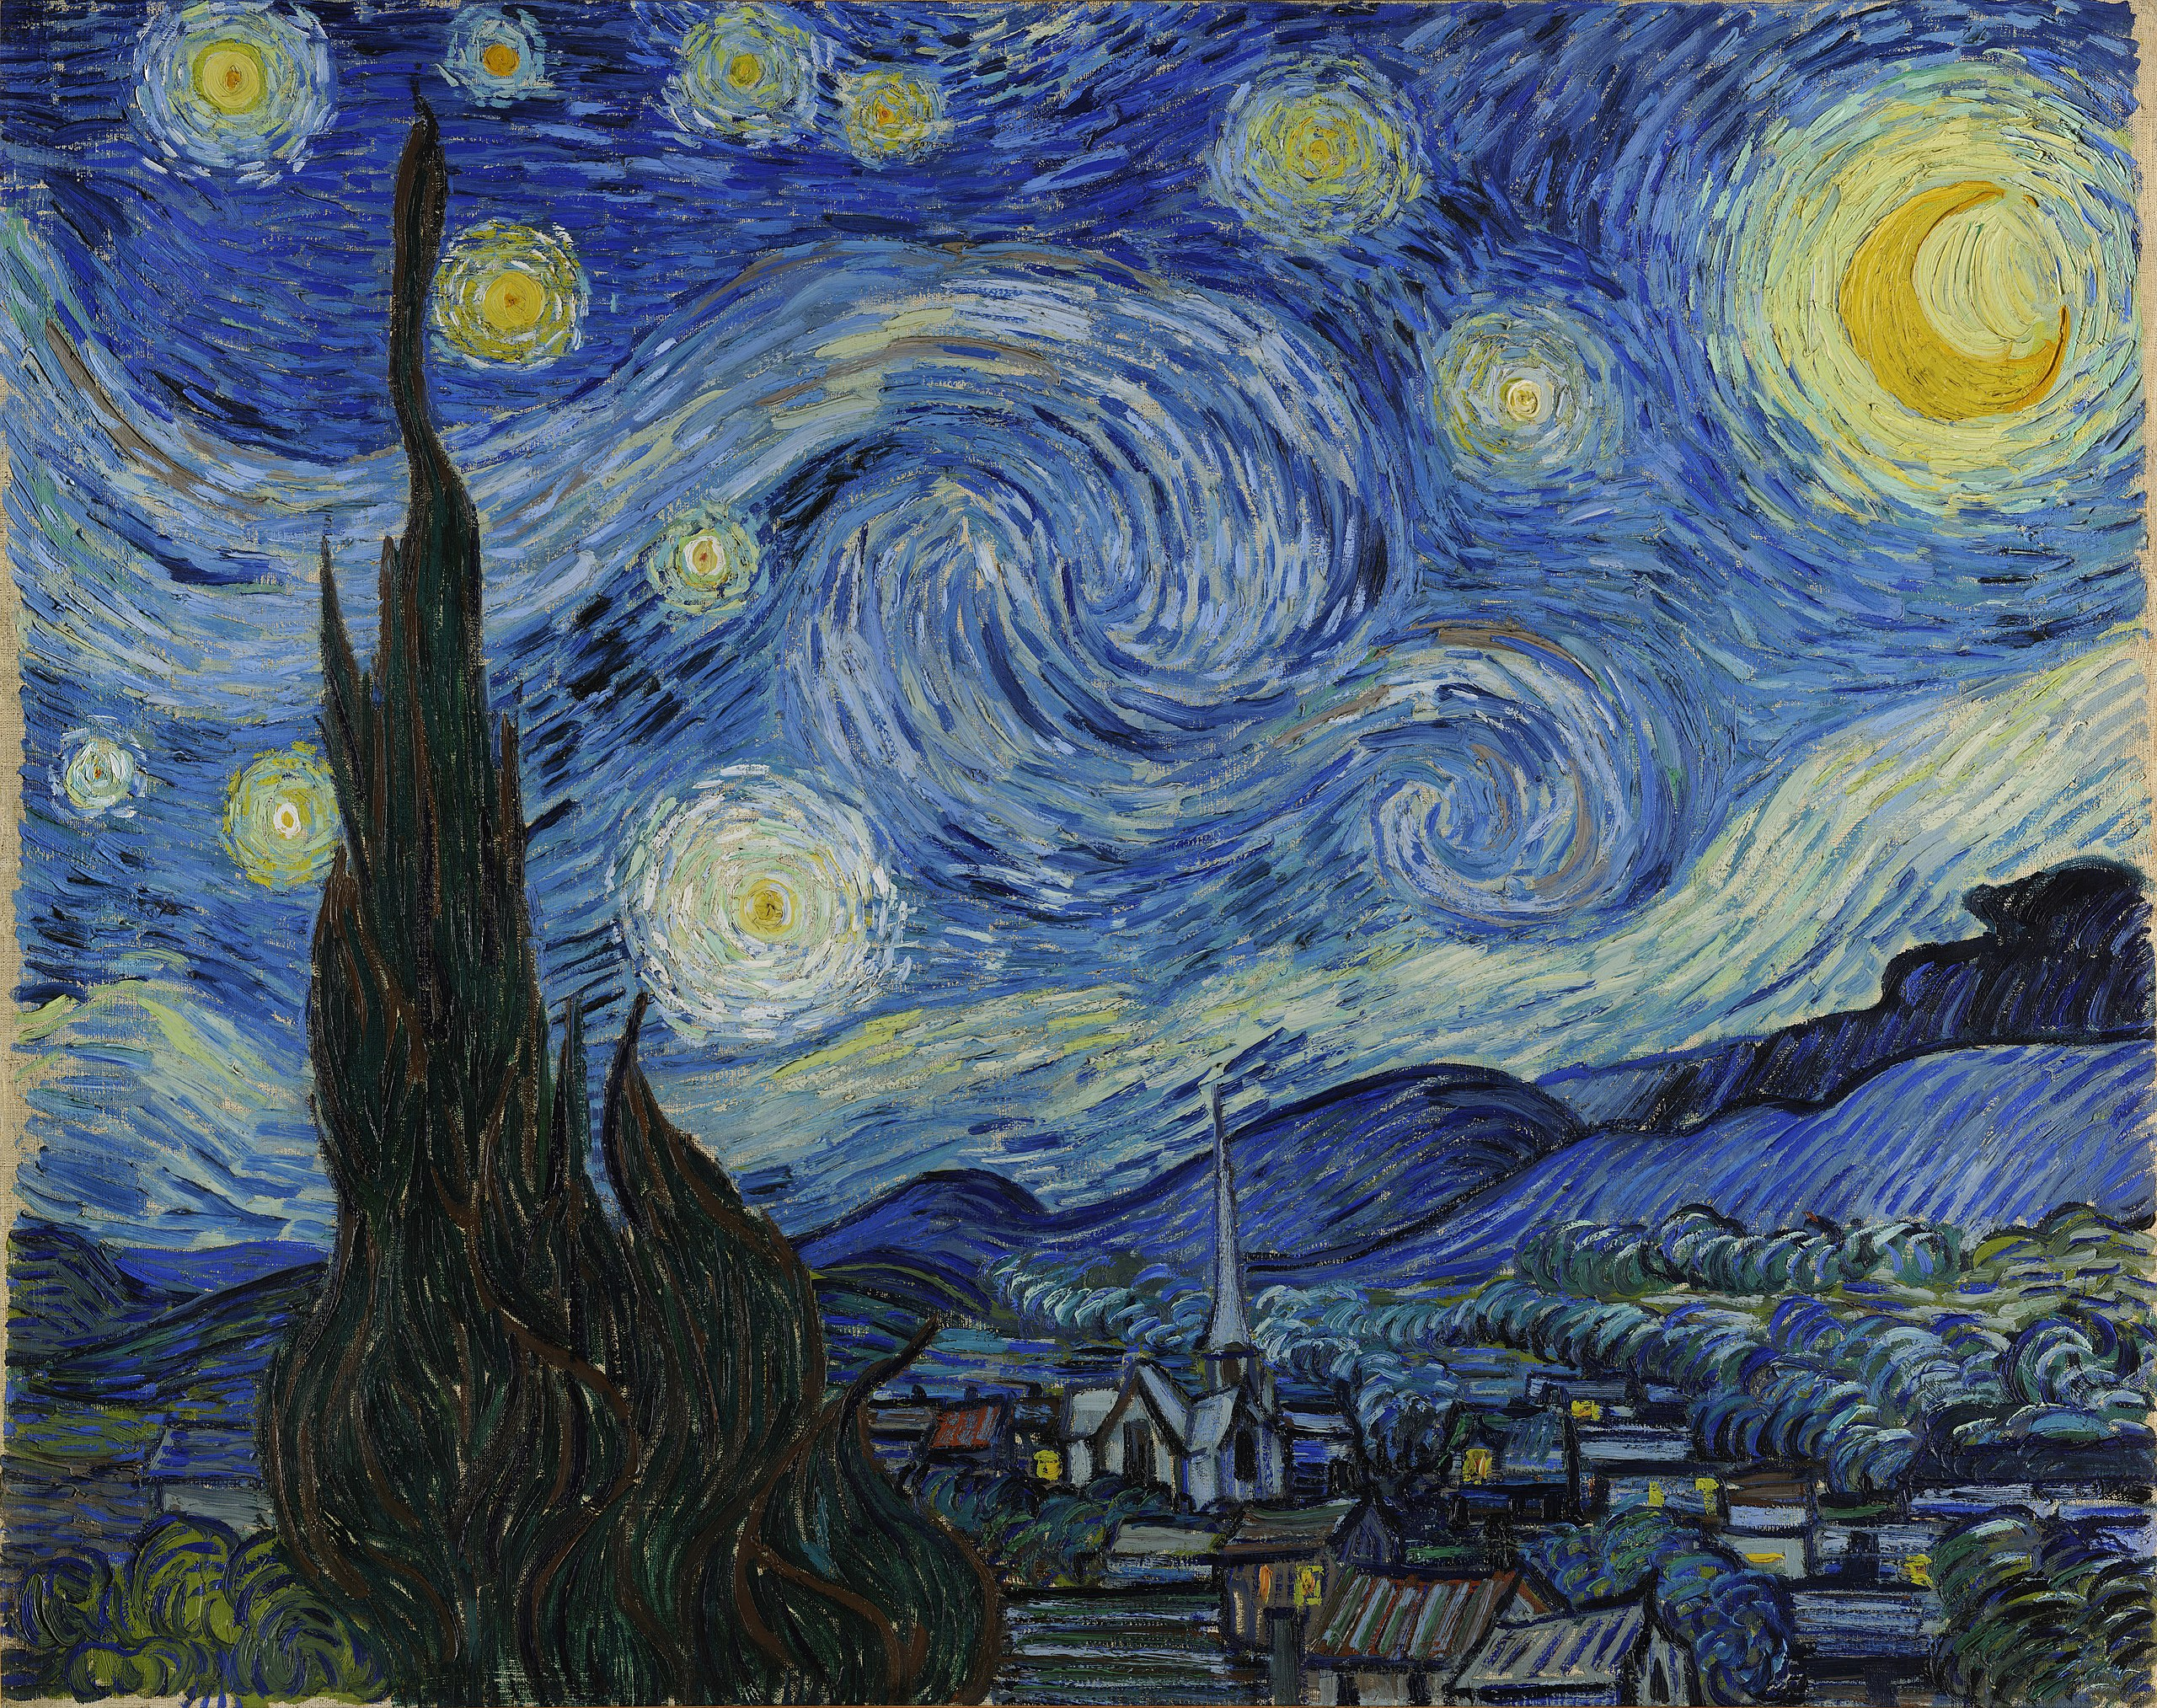
\includegraphics{figures/paintingexamples/starrynight}}
\caption{Like it or not, a continuous relation $[0,1] \rightarrow \blacksquare$: "The Starry Night", by Vincent van Gogh.}
\end{marginfigure}

\section{The category \textbf{TopRel}}

\begin{proposition}
Topological relations form a category $\mathbf{TopRel}$.
\begin{proof}
\newthought{Identities:} Identity relations, which are always topological.

\newthought{Composition:} The normal composition of relations. We verify that the composite $X^\tau \overset{R}{\rightarrow} Y^\sigma \overset{S}{\rightarrow} Z^\theta$ is again topological as follows:
\[U \in \theta \implies S^\dag(U) \in \sigma \implies R^\dag \circ S^\dag(U) = (S \circ R)^\dag \in \tau\]

\newthought{Associativity of composition:} Inherited from \textbf{Rel}.
\end{proof}
\end{proposition}

\section{Biproducts}

We exhibit a free-forgetful adjunction between \textbf{Rel} and \textbf{TopRel}.

\begin{defn}[F: $\mathbf{Rel} \rightarrow \mathbf{TopRel}$] We define the action of the functor $F$:
\begin{description}
\item[On objects] $F(X) := X^\star$, ($X$ with the discrete topology)
\item[On morphisms] $F(X \overset{R}{\rightarrow} Y) := X^\star \overset{R}{\rightarrow} Y^\star$. Recall that any relation between sets is continuous with respect to the discrete topology.
\end{description}
Evidently identities and associativity of composition are preserved.
\end{defn}

\begin{defn}[U: $\mathbf{TopRel} \rightarrow \mathbf{Rel}$]
\begin{description} We define the action of the functor $U$:
\item[On objects] $U(X^\tau) := X$
\item[On morphisms] $U(X^\tau \overset{R}{\rightarrow} Y^\sigma) := X \overset{R}{\rightarrow} Y$
\end{description}
Evidently identities and associativity of composition are preserved.
\end{defn}

\begin{proposition}[$F \dashv U \dashv F$]
\begin{proof}

By triangular identities.

The composite $FU$ is precisely equal to the identity functor on $\mathbf{Rel}$. The unit natural transformation $1_\mathbf{Rel} \Rightarrow FU$ we take to be the identity morphisms.

\[\eta_{X} := \text{id}_{X}\]

The counit natural transformation $UF \Rightarrow 1_{\mathbf{TopRel}}$ we define:

\[\epsilon_{X^\tau} : X^\star \rightarrow X^\tau := \{(x,x) : x \in X\}\]

Now we verify the triangle identities

\[\]

\end{proof}
\end{proposition}

\begin{corollary}
$\mathbf{TopRel}$ has a zero object and biproducts.
\begin{proof}

\end{proof}
\end{corollary}

\section{Symmetric Monoidal Closed structure}

\marginnote{
\begin{rem}[Product Topology]
We denote the product topology of $X^\tau$ and $Y^\sigma$ as $(X \times Y)^{(\tau \times \sigma)}$. $\tau \times \sigma$ is the topology on $X \times Y$ generated by the basis $\{t \times s : t \in \mathfrak{b}_\tau, s \in \mathfrak{b}_\sigma\}$, where $\mathfrak{b}_\tau$ and $\mathfrak{b}_\sigma$ are bases for $\tau$ and $\sigma$ respectively.
\end{rem}
}

\begin{proposition}
$(\mathbf{TopRel},\{\star\}^{\bullet},X^\tau \otimes Y^\sigma := (X \times Y)^{(\tau \times \sigma)})$ is a symmetric monoidal closed category.
\begin{proof}

\newthought{Tensor Unit:} The one-point space $\bullet$. Explicitly, $\{\star\}$ with topology $\{\varnothing,\{\star\}\}$.

\marginnote{
    \begin{rem}[Product of relations]
    For relations between sets $R: X \rightarrow Y, S: A \rightarrow B$, the product relation $R \times S: X \times A \rightarrow Y \times B$ is defined to be \[ \{ ((x,a),(y,b)) : (x,y) \in R, (a,b) \in S \} \]
    \end{rem}
}

\newthought{Tensor Product:} For objects, $X^\tau \otimes Y^\sigma$ has base set $X \times Y$ equipped with the product topology $\tau \times \sigma$. For morphisms, $R \otimes S$ the product of relations. We show that the tensor of continuous relations is again a continuous relation. Take continuous relations $R: X^\tau \rightarrow Y^\sigma$, $S: A^\alpha \rightarrow B^\beta$, and let $U$ be open in the product topology $(\sigma \times \beta)$. We need to prove that $(R \times S)^\dag(U) \in (\tau \times \alpha)$. We may express $U$ as $\bigcup\limits_{i \in I} y_i \times b_i$, where the $y_i$ and $b_i$ are in the bases $\mathfrak{b}_\sigma$ and $\mathfrak{b}_\beta$ respectively. Since for any relations we have that $R(A \cup B) = R(A) \cup R(B)$ and $(R \times S)^\dag = R^\dag \times S^\dag$:

\begin{align*}
&(R \times S)^\dag(\bigcup\limits_{i \in I} y_i \times b_i)\\
 &= \bigcup\limits_{i \in I}(R \times S)^\dag(y_i \times b_i)\\
 &= \bigcup\limits_{i \in I}(R^\dag \times S^\dag)(y_i \times b_i)
 \end{align*}

Since each $y_i$ is open and $R$ is continuous, $R^\dag(y_i) \in \tau$. Symmetrically, $S^\dag(b_i) \in \alpha$. So each $(R^\dag \times S^\dag)(y_i \times b_i) \in (\tau \times \alpha)$. Topologies are closed under arbitrary union, so we are done.

\newthought{Unitors:} The left unitors $\lambda_{X^{\tau}}: \bullet \times X^\tau \rightarrow X^\tau$ maps $(\star,x) \mapsto x$, and we reverse the direction of the mapping to obtain the inverse $\lambda^{-1}_{X^{\tau}}$. The construction is symmetric for the right unitors $\rho_{X^{\tau}}$. 

\newthought{Associators:}

The associators $\alpha_{X^{\tau},Y^{\sigma},Z^{\rho}}$

\newthought{Braids:}


\newthought{Coherences:}



\end{proof}
\end{proposition}

\section{States, Effects, Spiders}

\marginnote{
\begin{intuition}\label{intuit:screen}
View the space as a screen display, with points as pixels. Then states are "shapes" of lit up pixels, and effects are "tests", which check for lit pixels in an open set. In a discrete topology, all shapes are distinguishable by testing. In an indiscrete topology, the only distinction is between "no shape" and "some shape".
\end{intuition}
}



\subsection{When does an object have a spider (or something close to one)?}

\marginnote{
\begin{rem}[copy-compare spiders of $\mathbf{Rel}$]
For a set $X$, the \emph{copy} map $X \rightarrow X \times X$ is defined:
\[\{(x,(x,x)) : x \in X \}\]
the \emph{compare} map $X \times X \rightarrow X$ is defined:
\[\{((x,x),x) : x \in X \}\]
These two maps are the (co)multiplications of special frobenius algebras. The (co)units are \emph{delete}:
\[\{(x,\star) : x \in X\}\]
and \emph{everything}:
\[\{(\star,x) : x \in X\}\]
\end{rem}
}

\begin{example}[The copy-compare spiders of $\mathbf{Rel}$ are not always topological]\label{ex:compnotspider}
The compare map for the Sierpi\'{n}ski space is not topological, because the preimage of $\{0,1\}$ is $\{(0,0),(1,1)\}$, which is not open in the product space of $\mathcal{S}$ with itself.
\end{example}

\newthought{What do we want from a spider?} Arguably, the main thing we want from a spider the forcing of all of its inputs and outputs to be equal: "equating variables" is the earliest incarnation of spiders [CITE]. A comorbidity with spiders is the ability to efficiently or finitely represent morphisms with basis states and effects [CITE]. Finally, spiders admit an easy graphical calculus [CITE].\\

However, we have seen from Example \ref{ex:compnotspider} that the usual spiders from \textbf{Rel} do not work. Elaborating Intuition \ref{intuit:screen}, the usual spiders from \textbf{Rel} assume the discrete topology, which corresponds to a "perfect" ability to distinguish/recognise/encode shapes. So we are looking for a condition on the topology that still allows us to do all that, more or less.

\subsection{ Compact Hausdorff spaces are arachnid }

\marginnote{

\begin{rem}[Compactness]
An \textbf{open cover} of a space $X^\tau$ is a set of opens $\{U_i: i \in I\} \subset \tau$ such that:
\[ \bigcup\limits_{i \in I} U_i = X \]
A \textbf{subcover} of an open cover is a subset of the open cover that is still an open cover.
$X^\tau$ is \textbf{compact} when every open cover has a finite subcover.
\end{rem}

\begin{rem}[Hausdorff]
$X^\tau$ is \textbf{Hausdorff} when for any two distinct points $a,b \in X$ there are disjoint opens $U,V \in \tau$ such that $a \in U$ and $b \in V$. The mnemonic is that the points are "housed-off".
\end{rem}

}

\begin{defn}[Non-unital Spider]
A \textbf{non-unital spider} on $X^\tau$ is a tuple [[[placeholder]]] that satisfies the following relations:

\end{defn}

\begin{defn}[Arachnidity]
Call $X^\tau$ \textbf{arachnid} if it admits a family of non-unital spiders such that for any finite family $\mathbb{K}:=\{K_i \subset X : i \in I, \ |I| \in \mathbb{N}\}$ of subsets of $X$, there exists a non-unital spider on $X^\tau$ such that:

[[placeholder]]

\end{defn}

\begin{theorem}[Compact Hausdorff is Arachnidity]
$X^\tau$ is compact and Hausdorff iff $X^\tau$ is arachnid.
\end{theorem}

We prove this by first relating arachnidity to some conditions that are phrased in the "distinguishing shapes" setting of Intuition \ref{intuit:screen}, and then bridge to compact Hausdorff.

\subsection{Arachnidity, Distinguishing, Encoding, Recognition}

\newthought{When is the topology of a space "good"?} There are several possible criteria for "goodness", such as the ability to distinguish different shapes, encode those shapes in the results of testing, and reconstruct those shapes from an encoding.

\marginnote{
    \begin{remark}
        Where $\tau$ of all opens represents all possible tests, a test battery is a specific set of tests.
    \end{remark}
}
\begin{defn}[Test battery]
A \textbf{test battery} of $X^\tau$ is a subset of $\tau$.
\end{defn}
\marginnote{
    \begin{remark}
    A curriculum is a range of possible shapes.
    \end{remark}
}
\begin{defn}[Curriculum]
A \textbf{curriculum} of $X^\tau$ is a set of subsets of $X$.
\end{defn}

\marginnote{
\begin{remark}
If $X^\tau$ is not distinguishing, then there are two distinct shapes $J \neq K$ that no test can tell apart.
\end{remark}    
}
\begin{defn}[Distinguishing]\label{def:distinguish}
$X^\tau$ is \textbf{distinguishing} when
\[\forall J,K_{(\subseteq X)} (J \neq K \iff \exists U_{(\in \tau)}: placeholder)\]
\end{defn}

\marginnote{
    \begin{remark}
    An encoding is a binary spectrum; for each test in the battery, a bit indicating whether that test has failed or succeeded.
    \end{remark}
}
\begin{defn}[Encoding]
An \textbf{encoding} of $K \subset X$ with respect to a test battery $\mathbb{T}: \{U_i : i \in I, U_i \in \tau\}$ is a direct sum:
\[placeholder\]
\end{defn}

\marginnote{
    \begin{remark}
    A recogniser can take any finite curriculum and provide a finite test battery such that shapes can be distinguished via their finite encodings. Finiteness is a weak but necessary condition computability -- i.e. practical feasibility.
    \end{remark}
}
\begin{defn}[Recognition: computable distinguishing encodings]
$X^\tau$ is a \textbf{recogniser} if for any finite $\mathbb{K} := \{ K_i \subseteq X : i \in I, \ |I|\in \mathbb{N} \}$, there exists a finite test battery $\mathbb{U} := \{ U_j \in \tau: j \in J, \ |J|\in \mathbb{N} \} \subseteq \tau$ such that:
\[K_a \neq K_b \iff placeholder\]
\end{defn}

\marginnote{
    \begin{remark}
    Instead of providing a different test battery for each curriculum, it would be more convenient to extend the test battery whenever an unseen shape enters the curriculum; this is what a learner does.
    \end{remark}
}

\begin{defn}[Learning: extendable recognisers]
A recogniser is a \textbf{learner} when, for arbitrary finite curricula $\mathbb{K}' \supset \mathbb{K}$ and a finite test battery $\mathbb{U}$:
\[placeholder \iff \exists \mathbb{U}'_{(\mathbb{U} \subseteq \mathbb{U}' \subseteq \tau)}:( |\mathbb{U}'| \in \mathbb{N} \wedge placeholder)\]

\end{defn}

\marginnote{
    \begin{remark}
    Recall 
    \end{remark}
}
\begin{defn}[Recall: reconstruction from encodings]

\end{defn}

\marginnote{
    \begin{remark}

    \end{remark}
}

\begin{defn}

\end{defn}



\section{Enrichment structure}



Denote by $(X \times Y)^{(\tau \multimap \sigma)}$ the topological space of topological relations of type $X^\tau \rightarrow Y^\sigma$ as given above. We show that this topology is finer than the product topology.

\begin{proposition}
For any $X^\tau$ and $Y^\sigma$, $\tau \times \sigma \subseteq \tau \multimap \sigma$
\begin{proof}
Let $\mathfrak{b}_\tau, \mathfrak{b}_\sigma$ be bases for $\tau$ and $\sigma$ respectively, then $\tau \times \sigma$ has basis $\mathfrak{b}_\tau \times \mathfrak{b}_\sigma$. An arbitrarily element $(t \in \tau, s \in \sigma)$ of this product basis can be viewed as a topological relation $t \times s \subseteq X \times Y$. Every open of $\tau \times \sigma$ is a union of such basis elements, and topological relations are closed under arbitrary union, so we have the (evidently injective) correspondence:
\[ \tau \times \sigma \ni \bigcup\limits_{i \in I}(t_i \times s_i) \mapsto \bigcup\limits_{i \in I}(t_i \times s_i) \in \tau \multimap \sigma \]
\end{proof}
\end{proposition}

\marginnote{
\begin{example}[$\tau \multimap \sigma \nsubseteq \tau \times \sigma$]
Recalling Proposition \ref{prop:states}, let $\tau = \{\varnothing,\{\star\}\}$ on the singleton, and $\sigma$ be an arbitrary nondiscrete topology on base space Y. $(\{\star\} \times Y)^{(\tau \times \sigma)}$ is isomorphic to $Y^\sigma$, but $(\{\star\} \times Y)^{\tau \multimap \sigma)}$ is the isomorphic to the discrete topology $Y^\bullet$. For a more concrete example, consider the Sierpi\'{n}ski space $\mathcal{S}$ again, along with the topological relation $\{(0,0),(1,0),(1,1)\} \subset \mathcal{S} \times \mathcal{S}$; due to the presence of $(0,0)$, this topological relation cannot be formed by a union of basis elements of the product topology, which are:
\begin{description}
\item[$\{1\} \times \{1\}$ =] $\{(1,1)\}$
\item[$\{1\} \times \{0,1\}$ =] $\{ (1,0),(1,1) \}$
\item[$\{0,1\} \times \{1\}$ =] $\{ (1,1),(0,1) \}$
\item[$\{0,1\} \times \{0,1\}$ =] $\{ (0,0), (0,1), (1,0), (0,1) \}$
\end{description}

\end{example}
}

\begin{proposition}
$\tau \multimap \sigma = \tau \times \sigma \iff $
\begin{proof}

\end{proof}
\end{proposition}

\clearpage

\subsection{How \textbf{TopRel} relates to other well-known categories}

\[\begin{tikzcd}
    &&& {\mathbf{Loc}} \\
    \\
    \\
    {\mathbf{Top}} &&& {\mathbf{TopRel}} &&& {\mathbf{Rel}} \\
    \\
    \\
    &&& {\mathbf{Set}}
    \arrow[""{name=0, anchor=center, inner sep=0}, "{(-)_U}", curve={height=-12pt}, shorten <=8pt, shorten >=8pt, from=4-4, to=4-7]
    \arrow[""{name=1, anchor=center, inner sep=0}, "{(-)_D}", curve={height=-12pt}, shorten <=8pt, shorten >=8pt, from=4-7, to=4-4]
    \arrow[""{name=2, anchor=center, inner sep=0}, "{(-)_U}", curve={height=-12pt}, shorten <=10pt, shorten >=10pt, from=4-1, to=7-4]
    \arrow[""{name=3, anchor=center, inner sep=0}, "{(-)_D}", curve={height=-12pt}, shorten <=10pt, shorten >=10pt, from=7-4, to=4-1]
    \arrow[""{name=4, anchor=center, inner sep=0}, "{(-)_L}", curve={height=-12pt}, shorten <=10pt, shorten >=10pt, from=4-1, to=1-4]
    \arrow[""{name=5, anchor=center, inner sep=0}, "{(-)_P}", curve={height=-12pt}, shorten <=10pt, shorten >=10pt, from=1-4, to=4-1]
    \arrow[shorten <=5pt, shorten >=5pt, from=4-4, to=1-4]
    \arrow["i"{description}, shorten <=10pt, shorten >=10pt, hook, from=7-4, to=4-7]
    \arrow["i"{description}, shorten <=8pt, shorten >=8pt, hook, from=4-1, to=4-4]
    \arrow["\dashv"{anchor=center, rotate=45}, draw=none, from=3, to=2]
    \arrow["\dashv"{anchor=center, rotate=90}, draw=none, from=1, to=0]
    \arrow["\dashv"{anchor=center, rotate=-44}, draw=none, from=4, to=5]
\end{tikzcd}\]

Here are two ways to think about \textbf{TopRel} in relation to other categories. First, we can think of the analogy
\[\mathbf{TopRel}:\mathbf{Rel}::\mathbf{Top}:\mathbf{Set}\]
This analogy holds up to the free-forgetful adjunction between \textbf{Top} and \textbf{Set} embedding into a free-forgetful adjunction between \textbf{TopRel} and \textbf{Rel}.\marginnote{
    \begin{remark}[\textbf{TopRel} is not Kleisli in the obvious way]
    However, while \textbf{Rel} is the Kleisli category of \textbf{Set} with respect to the powerset monad, \textbf{TopRel} doesn't seem to be the Kleisli category of \textbf{Top} in an analogous way. The obvious notion of a powerset topology $\mathcal{P}\tau := \{S \subset \tau : \bigcup S \in \tau\}$ agrees with our na\"{i}ve definition of continuous relation, but the underlying unit and multiplication maps from the powerset monad on \textbf{Set} fail to be continuous with respect to this topology.
    \end{remark}
}



\begin{proposition}[\textbf{Rel} and \textbf{TopRel} free-forgetful adjunction]

\begin{proof}

\end{proof}
\end{proposition}


\begin{proposition}[(Outer square)]

\begin{proof}

\end{proof}
\end{proposition}

\begin{rem}[Locales, and the \textbf{Top}-\textbf{Loc} adjunction]

\end{rem}

\begin{proposition}[(Inner square)]

\begin{proof}

\end{proof}
\end{proposition}


\end{document}